\documentclass[a4paper,english,10pt]{article}\usepackage[]{graphicx}\usepackage[]{color}
%% maxwidth is the original width if it is less than linewidth
%% otherwise use linewidth (to make sure the graphics do not exceed the margin)
\makeatletter
\def\maxwidth{ %
  \ifdim\Gin@nat@width>\linewidth
    \linewidth
  \else
    \Gin@nat@width
  \fi
}
\makeatother

\definecolor{fgcolor}{rgb}{0.196, 0.196, 0.196}
\newcommand{\hlnum}[1]{\textcolor[rgb]{0.063,0.58,0.627}{#1}}%
\newcommand{\hlstr}[1]{\textcolor[rgb]{0.063,0.58,0.627}{#1}}%
\newcommand{\hlcom}[1]{\textcolor[rgb]{0.588,0.588,0.588}{#1}}%
\newcommand{\hlopt}[1]{\textcolor[rgb]{0.196,0.196,0.196}{#1}}%
\newcommand{\hlstd}[1]{\textcolor[rgb]{0.196,0.196,0.196}{#1}}%
\newcommand{\hlkwa}[1]{\textcolor[rgb]{0.231,0.416,0.784}{#1}}%
\newcommand{\hlkwb}[1]{\textcolor[rgb]{0.627,0,0.314}{#1}}%
\newcommand{\hlkwc}[1]{\textcolor[rgb]{0,0.631,0.314}{#1}}%
\newcommand{\hlkwd}[1]{\textcolor[rgb]{0.78,0.227,0.412}{#1}}%
\let\hlipl\hlkwb

\usepackage{framed}
\makeatletter
\newenvironment{kframe}{%
 \def\at@end@of@kframe{}%
 \ifinner\ifhmode%
  \def\at@end@of@kframe{\end{minipage}}%
  \begin{minipage}{\columnwidth}%
 \fi\fi%
 \def\FrameCommand##1{\hskip\@totalleftmargin \hskip-\fboxsep
 \colorbox{shadecolor}{##1}\hskip-\fboxsep
     % There is no \\@totalrightmargin, so:
     \hskip-\linewidth \hskip-\@totalleftmargin \hskip\columnwidth}%
 \MakeFramed {\advance\hsize-\width
   \@totalleftmargin\z@ \linewidth\hsize
   \@setminipage}}%
 {\par\unskip\endMakeFramed%
 \at@end@of@kframe}
\makeatother

\definecolor{shadecolor}{rgb}{.97, .97, .97}
\definecolor{messagecolor}{rgb}{0, 0, 0}
\definecolor{warningcolor}{rgb}{1, 0, 1}
\definecolor{errorcolor}{rgb}{1, 0, 0}
\newenvironment{knitrout}{}{} % an empty environment to be redefined in TeX

\usepackage{alltt}
\usepackage{a4a}
%\VignetteIndexEntry{Natural Mortality}
%\VignetteEngine{knitr::knitr}
\IfFileExists{upquote.sty}{\usepackage{upquote}}{}
\begin{document}

\title{Assessment for All initiative(a4a) \\ Natural Mortality Modelling}

\author[1]{Ernesto Jardim}
\author[1,2,3]{Colin Millar}
\author[1]{Finlay Scott}
\author[1]{Chato Osio}
\author[1]{Iago Mosqueira}
\affil[1]{European Commission, Joint Research Centre, Sustainable resources directorate, Water and Marine Resources unit, 21027 Ispra (VA), Italy}
\affil[2]{Marine Scotland Freshwater Laboratory, Faskally, Pitlochry, Perthshire PH16 5LB, UK}
\affil[3]{International Council for the Exploration of the Sea (ICES), H. C. Andersens Boulevard 44-46, 1553 Copenhagen V, Denmark}
\affil[*]{Corresponding author \href{mailto:ernesto.jardim@jrc.ec.europa.eu}{ernesto.jardim@jrc.ec.europa.eu}}



\maketitle

\abstract{The document explains the approach being developed by a4a to integrate uncertainty in natural mortality into stock assessment and advice. It presents a mixture of text and code, where the first explains the concepts behind the methods, while the last shows how these can be run with the software provided.}

\newpage
\tableofcontents
\newpage



\section{Background}

In the \aFa natural mortality is dealt with as an external parameter to the stock assessment model. The rationale to modelling natural mortality is similar to that of growth: one should be able to grab information from a range of sources and feed it into the assessment.

The mechanism used by \aFa is to build an interface that makes it transparent, flexible and hopefully easy to explore different options. In relation to natural mortality it means that the analyst should be able to use distinct models like Gislasson's, Charnov's, Pauly's, etc in a coherent framework making it possible to compare the outcomes of the assessment. 

Within the \aFa framework, the general method for inserting natural mortality in the stock assessment is to:

\begin{itemize}
    \item Create an object of class \class{a4aM} which holds the natural mortality model and parameters.
    \item Add uncertainty to the parameters in the \class{a4aM} object.
    \item Apply the \code{m()} method to the \class{a4aM} object to create an age or length based \class{FLQuant} object of the required dimensions.
\end{itemize}

The resulting \class{FLQuant} object can then be directly inserted into an \class {FLStock} object to be used for the assessment.   

In this section we go through each of the steps in detail using a variety of different models.

\section{License, documentation and development status}

The software is released under the \href{https://joinup.ec.europa.eu/community/eupl/home}{EUPL 1.1}.

For more information on the \aFa methodologies refer to \href{http://icesjms.oxfordjournals.org/content/early/2014/04/03/icesjms.fsu050.abstract}{Jardim, et.al, 2014}, \href{http://icesjms.oxfordjournals.org/content/early/2014/03/31/icesjms.fsu043.abstract}{Millar, et.al, 2014} and \href{http://journals.plos.org/plosone/article?id=10.1371/journal.pone.0154922}{Scott, et.al, 2016}.

Documentation can be found at \url{http://flr-project.org/FLa4a}. You are welcome to:

\begin{itemize}
	\item Submit suggestions and bug-reports at: \url{https://github.com/flr/FLa4a/issues}
	\item Send a pull request on: \url{https://github.com/flr/FLa4a/}
	\item Compose a friendly e-mail to the maintainer, see `packageDescription('FLa4a')`
\end{itemize}




%% ======================================
%% Call child document with libs and data

\section{Installing and loading libraries}

To run the \pkg{FLa4a} methods the reader will need to install the package and its dependencies and load them. Some datasets are distributed with the package and as such need to be loaded too.

\begin{knitrout}
\definecolor{shadecolor}{rgb}{0.949, 0.949, 0.949}\color{fgcolor}\begin{kframe}
\begin{alltt}
\hlcom{# from CRAN}
\hlkwd{install.packages}\hlstd{(}\hlkwd{c}\hlstd{(}\hlstr{"copula"}\hlstd{,} \hlstr{"triangle"}\hlstd{,} \hlstr{"coda"}\hlstd{))}
\hlcom{# from FLR}
\hlkwd{install.packages}\hlstd{(}\hlkwd{c}\hlstd{(}\hlstr{"FLCore"}\hlstd{,} \hlstr{"FLa4a"}\hlstd{),} \hlkwc{repos} \hlstd{=} \hlstr{"http://flr-project.org/R"}\hlstd{)}
\end{alltt}
\end{kframe}
\end{knitrout}

\begin{knitrout}
\definecolor{shadecolor}{rgb}{0.949, 0.949, 0.949}\color{fgcolor}\begin{kframe}
\begin{alltt}
\hlcom{# libraries}
\hlkwd{library}\hlstd{(FLa4a)}
\hlkwd{library}\hlstd{(XML)}
\hlkwd{library}\hlstd{(reshape2)}
\hlkwd{library}\hlstd{(latticeExtra)}
\hlcom{# datasets}
\hlkwd{data}\hlstd{(ple4)}
\hlkwd{data}\hlstd{(ple4.indices)}
\hlkwd{data}\hlstd{(ple4.index)}
\hlkwd{data}\hlstd{(rfLen)}
\end{alltt}
\end{kframe}
\end{knitrout}

\begin{knitrout}
\definecolor{shadecolor}{rgb}{0.949, 0.949, 0.949}\color{fgcolor}\begin{kframe}
\begin{alltt}
\hlkwd{packageVersion}\hlstd{(}\hlstr{"FLCore"}\hlstd{)}
\end{alltt}
\begin{verbatim}
## [1] '2.6.5.9005'
\end{verbatim}
\begin{alltt}
\hlkwd{packageVersion}\hlstd{(}\hlstr{"FLa4a"}\hlstd{)}
\end{alltt}
\begin{verbatim}
## [1] '2.0.0'
\end{verbatim}
\end{kframe}
\end{knitrout}



\section{How to read this document}

The target audience for this document are readers with some experience in R and some background on stock assessment.

The document explains the approach being developed by \aFa for fish stock assessment and scientific advice. It presents a mixture of text and code, where the first explains the concepts behind the methods, while the last shows how these can be run with the software provided. Moreover, having the code allows the reader to copy/paste and replicate the analysis presented here.

The sections and subsections are as independent as possible, so it can be used as a reference document for the \pkg{FLa4a}. 

%Section~\ref{sec:in} deals with reading and preparing data in \pkg{FLR} objects, which constitute the basic dataset for stock assessment with length structured models. This section is independent from \pkg{FLa4a} and relies mostly on \R and \pkg{reshape}.

%Sections~\ref{sec:l2a},\ref{sec:M} and \ref{sec:sca} are related with \pkg{FLa4a} and describe the concepts described in the previous section.

Finally, this is a live document which will be updated and released often.



\section{\code{a4aM} - The M class}

Natural mortality is implemented in a class named \class{a4aM}. This class is made up of three objects of the class \class{FLModelSim}. Each object is a model that represents one effect: an age or length effect, a scaling (level) effect and a time trend, named \code{shape}, \code{level} and \code{trend}, respectively. The impact of the models is multiplicative, i.e. the overal natural mortality is given by \class{shape} x  \class{level} x \class{trend}. Check the help files for more information.

\begin{knitrout}
\definecolor{shadecolor}{rgb}{0.949, 0.949, 0.949}\color{fgcolor}\begin{kframe}
\begin{alltt}
\hlkwd{showClass}\hlstd{(}\hlstr{"a4aM"}\hlstd{)}
\end{alltt}
\begin{verbatim}
## Class "a4aM" [package "FLa4a"]
## 
## Slots:
##                                                                         
## Name:       shape      level      trend       name       desc      range
## Class: FLModelSim FLModelSim FLModelSim  character  character    numeric
## 
## Extends: "FLComp"
\end{verbatim}
\end{kframe}
\end{knitrout}

The \class{a4aM} constructor requires that the models and parameters are provided. The default method will build each of these models as a constant value of 1.

As a simple example, the usual "0.2" guessestimate could be set up by setting the \code{level} model to have a single parameter with a fixed value, while the other two models, \class{shape} and \class{trend}, have a default value of 1 (meaning that they have no effect).

\begin{knitrout}
\definecolor{shadecolor}{rgb}{0.949, 0.949, 0.949}\color{fgcolor}\begin{kframe}
\begin{alltt}
\hlstd{mod02} \hlkwb{<-} \hlkwd{FLModelSim}\hlstd{(}\hlkwc{model} \hlstd{=} \hlopt{~}\hlstd{a,} \hlkwc{params} \hlstd{=} \hlkwd{FLPar}\hlstd{(}\hlkwc{a} \hlstd{=} \hlnum{0.2}\hlstd{))}
\hlstd{m1} \hlkwb{<-} \hlkwd{a4aM}\hlstd{(}\hlkwc{level} \hlstd{= mod02)}
\hlstd{m1}
\end{alltt}
\begin{verbatim}
## a4aM object:
##   shape: ~1
##   level: ~a
##   trend: ~1
\end{verbatim}
\end{kframe}
\end{knitrout}

More interesting natural mortality shapes can be set up using biological knowledge. The following example uses an exponential decay over ages (implying that the resulting \class{FLQuant} generated by the \code{m()} method will be age based). We also use Jensen's second estimator (\href{http://onlinelibrary.wiley.com/doi/10.1111/faf.12027/abstract}{Kenchington, 2014}) as a scaling \code{level} model, which is based on the von Bertalanffy $K$ parameter, $M=1.5K$. 

\begin{knitrout}
\definecolor{shadecolor}{rgb}{0.949, 0.949, 0.949}\color{fgcolor}\begin{kframe}
\begin{alltt}
\hlstd{shape2} \hlkwb{<-} \hlkwd{FLModelSim}\hlstd{(}\hlkwc{model} \hlstd{=} \hlopt{~}\hlkwd{exp}\hlstd{(}\hlopt{-}\hlstd{age} \hlopt{-} \hlnum{0.5}\hlstd{))}
\hlstd{level2} \hlkwb{<-} \hlkwd{FLModelSim}\hlstd{(}\hlkwc{model} \hlstd{=} \hlopt{~}\hlnum{1.5} \hlopt{*} \hlstd{k,} \hlkwc{params} \hlstd{=} \hlkwd{FLPar}\hlstd{(}\hlkwc{k} \hlstd{=} \hlnum{0.4}\hlstd{))}
\hlstd{m2} \hlkwb{<-} \hlkwd{a4aM}\hlstd{(}\hlkwc{shape} \hlstd{= shape2,} \hlkwc{level} \hlstd{= level2)}
\hlstd{m2}
\end{alltt}
\begin{verbatim}
## a4aM object:
##   shape: ~exp(-age - 0.5)
##   level: ~1.5 * k
##   trend: ~1
\end{verbatim}
\end{kframe}
\end{knitrout}

Note that the \code{shape} model has \code{age} as a parameter of the model but is not set using the \code{params} argument.

The \code{shape} model does not have to be age-based. For example, here we set up a \code{shape} model using Gislason's second estimator (\href{}{Kenshington, 2013}):
$M_l=K(\frac{L_{\inf}}{l})^{1.5}$. We use the default \code{level} and \class{trend} models.
% Current m() method is not ideal for length based methods as you cannot specify length range and half-widths to make compatible with FLStockLen

\begin{knitrout}
\definecolor{shadecolor}{rgb}{0.949, 0.949, 0.949}\color{fgcolor}\begin{kframe}
\begin{alltt}
\hlstd{shape_len} \hlkwb{<-} \hlkwd{FLModelSim}\hlstd{(}\hlkwc{model} \hlstd{=} \hlopt{~}\hlstd{K} \hlopt{*} \hlstd{(linf}\hlopt{/}\hlstd{len)}\hlopt{^}\hlnum{1.5}\hlstd{,} \hlkwc{params} \hlstd{=} \hlkwd{FLPar}\hlstd{(}\hlkwc{linf} \hlstd{=} \hlnum{60}\hlstd{,}
    \hlkwc{K} \hlstd{=} \hlnum{0.4}\hlstd{))}
\hlstd{m_len} \hlkwb{<-} \hlkwd{a4aM}\hlstd{(}\hlkwc{shape} \hlstd{= shape_len)}
\end{alltt}
\end{kframe}
\end{knitrout}

Another option is to model how an external factor may impact the natural mortality. This can be added through the \code{trend} model. Suppose natural mortality can be modelled with a dependency on the NAO index, due to some mechanism that results in having lower mortality when NAO is negative and higher when it's positive. In this example, the impact is represented by the NAO value on the quarter before spawning, which occurs in the second quarter. 

We use this to make a complicated natural mortality model with an age based shape model, a level model based on $K$ and a trend model driven by NAO, where mortality increases by 50\% if NAO is positive on the first quarter.

\begin{knitrout}
\definecolor{shadecolor}{rgb}{0.949, 0.949, 0.949}\color{fgcolor}\begin{kframe}
\begin{alltt}
\hlcom{# Get NAO}
\hlstd{nao.orig} \hlkwb{<-} \hlkwd{read.table}\hlstd{(}\hlstr{"https://www.esrl.noaa.gov/psd/data/correlation/nao.data"}\hlstd{,}
    \hlkwc{skip} \hlstd{=} \hlnum{1}\hlstd{,} \hlkwc{nrow} \hlstd{=} \hlnum{62}\hlstd{,} \hlkwc{na.strings} \hlstd{=} \hlstr{"-99.90"}\hlstd{)}
\hlstd{dnms} \hlkwb{<-} \hlkwd{list}\hlstd{(}\hlkwc{quant} \hlstd{=} \hlstr{"nao"}\hlstd{,} \hlkwc{year} \hlstd{=} \hlnum{1948}\hlopt{:}\hlnum{2009}\hlstd{,} \hlkwc{unit} \hlstd{=} \hlstr{"unique"}\hlstd{,} \hlkwc{season} \hlstd{=} \hlnum{1}\hlopt{:}\hlnum{12}\hlstd{,}
    \hlkwc{area} \hlstd{=} \hlstr{"unique"}\hlstd{)}
\hlcom{# Build an FLQuant from the NAO data}
\hlstd{nao.flq} \hlkwb{<-} \hlkwd{FLQuant}\hlstd{(}\hlkwd{unlist}\hlstd{(nao.orig[,} \hlopt{-}\hlnum{1}\hlstd{]),} \hlkwc{dimnames} \hlstd{= dnms,} \hlkwc{units} \hlstd{=} \hlstr{"nao"}\hlstd{)}
\hlcom{# Build covar by calculating mean over the first 3 months}
\hlstd{nao} \hlkwb{<-} \hlkwd{seasonMeans}\hlstd{(nao.flq[, , ,} \hlnum{1}\hlopt{:}\hlnum{3}\hlstd{])}
\hlcom{# Turn into Boolean}
\hlstd{nao} \hlkwb{<-} \hlstd{(nao} \hlopt{>} \hlnum{0}\hlstd{)}
\hlcom{# Constructor}
\hlstd{trend3} \hlkwb{<-} \hlkwd{FLModelSim}\hlstd{(}\hlkwc{model} \hlstd{=} \hlopt{~}\hlnum{1} \hlopt{+} \hlstd{b} \hlopt{*} \hlstd{nao,} \hlkwc{params} \hlstd{=} \hlkwd{FLPar}\hlstd{(}\hlkwc{b} \hlstd{=} \hlnum{0.5}\hlstd{))}
\hlstd{shape3} \hlkwb{<-} \hlkwd{FLModelSim}\hlstd{(}\hlkwc{model} \hlstd{=} \hlopt{~}\hlkwd{exp}\hlstd{(}\hlopt{-}\hlstd{age} \hlopt{-} \hlnum{0.5}\hlstd{))}
\hlstd{level3} \hlkwb{<-} \hlkwd{FLModelSim}\hlstd{(}\hlkwc{model} \hlstd{=} \hlopt{~}\hlnum{1.5} \hlopt{*} \hlstd{k,} \hlkwc{params} \hlstd{=} \hlkwd{FLPar}\hlstd{(}\hlkwc{k} \hlstd{=} \hlnum{0.4}\hlstd{))}
\hlstd{m3} \hlkwb{<-} \hlkwd{a4aM}\hlstd{(}\hlkwc{shape} \hlstd{= shape3,} \hlkwc{level} \hlstd{= level3,} \hlkwc{trend} \hlstd{= trend3)}
\hlstd{m3}
\end{alltt}
\begin{verbatim}
## a4aM object:
##   shape: ~exp(-age - 0.5)
##   level: ~1.5 * k
##   trend: ~1 + b * nao
\end{verbatim}
\end{kframe}
\end{knitrout}

\section{Adding uncertainty to natural mortality parameters with a multivariate normal distribution}

Uncertainty on natural mortality is added through uncertainty on the parameters.

In this section we'll' show how to add multivariate normal uncertainty. We make use of the class \class{FLModelSim} method \code{mvrnorm()}, which is a wrapper for the method \code{mvrnorm()} distributed by the package \pkg{MASS}.

We'll create an \class{a4aM} object with an exponential shape, a \code{level} model based on $k$ and temperature (Jensen's third estimator), and a \code{trend} model driven by the NAO (as above). Afterwards a variance-covariance matrix for the \code{level} and \code{trend} models will be included. Finally, create an object with 100 iterations using the \code{mvrnorm()} method.

Create the object:

\begin{knitrout}
\definecolor{shadecolor}{rgb}{0.949, 0.949, 0.949}\color{fgcolor}\begin{kframe}
\begin{alltt}
\hlstd{shape4} \hlkwb{<-} \hlkwd{FLModelSim}\hlstd{(}\hlkwc{model} \hlstd{=} \hlopt{~}\hlkwd{exp}\hlstd{(}\hlopt{-}\hlstd{age} \hlopt{-} \hlnum{0.5}\hlstd{))}
\hlstd{level4} \hlkwb{<-} \hlkwd{FLModelSim}\hlstd{(}\hlkwc{model} \hlstd{=} \hlopt{~}\hlstd{k}\hlopt{^}\hlnum{0.66} \hlopt{*} \hlstd{t}\hlopt{^}\hlnum{0.57}\hlstd{,} \hlkwc{params} \hlstd{=} \hlkwd{FLPar}\hlstd{(}\hlkwc{k} \hlstd{=} \hlnum{0.4}\hlstd{,} \hlkwc{t} \hlstd{=} \hlnum{10}\hlstd{),}
    \hlkwc{vcov} \hlstd{=} \hlkwd{array}\hlstd{(}\hlkwd{c}\hlstd{(}\hlnum{0.002}\hlstd{,} \hlnum{0.01}\hlstd{,} \hlnum{0.01}\hlstd{,} \hlnum{1}\hlstd{),} \hlkwc{dim} \hlstd{=} \hlkwd{c}\hlstd{(}\hlnum{2}\hlstd{,} \hlnum{2}\hlstd{)))}
\hlstd{trend4} \hlkwb{<-} \hlkwd{FLModelSim}\hlstd{(}\hlkwc{model} \hlstd{=} \hlopt{~}\hlnum{1} \hlopt{+} \hlstd{b} \hlopt{*} \hlstd{nao,} \hlkwc{params} \hlstd{=} \hlkwd{FLPar}\hlstd{(}\hlkwc{b} \hlstd{=} \hlnum{0.5}\hlstd{),} \hlkwc{vcov} \hlstd{=} \hlkwd{matrix}\hlstd{(}\hlnum{0.02}\hlstd{))}
\hlstd{m4} \hlkwb{<-} \hlkwd{a4aM}\hlstd{(}\hlkwc{shape} \hlstd{= shape4,} \hlkwc{level} \hlstd{= level4,} \hlkwc{trend} \hlstd{= trend4)}
\hlcom{# Call mvrnorm()}
\hlstd{m4} \hlkwb{<-} \hlkwd{mvrnorm}\hlstd{(}\hlnum{100}\hlstd{, m4)}
\hlstd{m4}
\end{alltt}
\begin{verbatim}
## a4aM object:
##   shape: ~exp(-age - 0.5)
##   level: ~k^0.66 * t^0.57
##   trend: ~1 + b * nao
\end{verbatim}
\end{kframe}
\end{knitrout}

Inspect the level model (for example):

\begin{knitrout}
\definecolor{shadecolor}{rgb}{0.949, 0.949, 0.949}\color{fgcolor}\begin{kframe}
\begin{alltt}
\hlstd{m4}\hlopt{@}\hlkwc{level}
\end{alltt}
\begin{verbatim}
## An object of class "FLModelSim"
## Slot "model":
## ~k^0.66 * t^0.57
## 
## Slot "params":
## An object of class "FLPar"
## iters:  100 
## 
## params
##               k               t 
## 0.39104(0.0375) 9.67575(0.9246) 
## units:  NA 
## 
## Slot "vcov":
##       [,1] [,2]
## [1,] 0.002 0.01
## [2,] 0.010 1.00
## 
## Slot "distr":
## [1] "norm"
\end{verbatim}
\end{kframe}
\end{knitrout}

Note the variance in the parameters: 

\begin{knitrout}
\definecolor{shadecolor}{rgb}{0.949, 0.949, 0.949}\color{fgcolor}\begin{kframe}
\begin{alltt}
\hlkwd{params}\hlstd{(}\hlkwd{trend}\hlstd{(m4))}
\end{alltt}
\begin{verbatim}
## An object of class "FLPar"
## iters:  100 
## 
## params
##              b 
## 0.50718(0.159) 
## units:  NA
\end{verbatim}
\end{kframe}
\end{knitrout}

Note the shape model has no parameters and no uncertainty:

\begin{knitrout}
\definecolor{shadecolor}{rgb}{0.949, 0.949, 0.949}\color{fgcolor}\begin{kframe}
\begin{alltt}
\hlkwd{params}\hlstd{(}\hlkwd{shape}\hlstd{(m4))}
\end{alltt}
\begin{verbatim}
## An object of class "FLPar"
## [1] NA
## units:  NA
\end{verbatim}
\end{kframe}
\end{knitrout}

In this particular case, the \code{shape} model will not be randomized because it doesn't have a variance-covariance matrix. Also note that because there is only one parameter in the \code{trend} model, the randomization will use a univariate normal distribution.

The same model could be achieved by using \code{mnrnorm()} on each model component:

\begin{knitrout}
\definecolor{shadecolor}{rgb}{0.949, 0.949, 0.949}\color{fgcolor}\begin{kframe}
\begin{alltt}
\hlstd{m4} \hlkwb{<-} \hlkwd{a4aM}\hlstd{(}\hlkwc{shape} \hlstd{= shape4,} \hlkwc{level} \hlstd{=} \hlkwd{mvrnorm}\hlstd{(}\hlnum{100}\hlstd{, level4),} \hlkwc{trend} \hlstd{=} \hlkwd{mvrnorm}\hlstd{(}\hlnum{100}\hlstd{,}
    \hlstd{trend4))}
\end{alltt}
\end{kframe}
\end{knitrout}

%Note: How to include ageing error ???

\section{Adding uncertainty to natural mortality parameters with statistical copulas}

We can also use copulas to add parameter uncertainty to the natural mortality model, similar to the way we use them for the growth model in Section \ref{sec:growth_triangle_cop}. As stated above these processes make use of the methods implemented for the \class{FLModelSim} class.

% EXPAND...

In the following example we'll use again Gislason's second estimator, $M_l=K(\frac{L_{\inf}}{l})^{1.5}$ and a triangle copula to model parameter uncertainty. The method \code{mvrtriangle()} is used to create 1000 iterations. 

\begin{knitrout}
\definecolor{shadecolor}{rgb}{0.949, 0.949, 0.949}\color{fgcolor}\begin{kframe}
\begin{alltt}
\hlstd{linf} \hlkwb{<-} \hlnum{60}
\hlstd{k} \hlkwb{<-} \hlnum{0.4}
\hlcom{# vcov matrix (make up some values)}
\hlstd{mm} \hlkwb{<-} \hlkwd{matrix}\hlstd{(}\hlnum{NA}\hlstd{,} \hlkwc{ncol} \hlstd{=} \hlnum{2}\hlstd{,} \hlkwc{nrow} \hlstd{=} \hlnum{2}\hlstd{)}
\hlcom{# 10% cv}
\hlkwd{diag}\hlstd{(mm)} \hlkwb{<-} \hlkwd{c}\hlstd{((linf} \hlopt{*} \hlnum{0.1}\hlstd{)}\hlopt{^}\hlnum{2}\hlstd{, (k} \hlopt{*} \hlnum{0.1}\hlstd{)}\hlopt{^}\hlnum{2}\hlstd{)}
\hlcom{# 0.2 correlation}
\hlstd{mm[}\hlkwd{upper.tri}\hlstd{(mm)]} \hlkwb{<-} \hlstd{mm[}\hlkwd{lower.tri}\hlstd{(mm)]} \hlkwb{<-} \hlkwd{c}\hlstd{(}\hlnum{0.05}\hlstd{)}
\hlcom{# a good way to check is using cov2cor}
\hlkwd{cov2cor}\hlstd{(mm)}
\end{alltt}
\begin{verbatim}
##           [,1]      [,2]
## [1,] 1.0000000 0.2083333
## [2,] 0.2083333 1.0000000
\end{verbatim}
\begin{alltt}
\hlcom{# create object}
\hlstd{mgis2} \hlkwb{<-} \hlkwd{FLModelSim}\hlstd{(}\hlkwc{model} \hlstd{=} \hlopt{~}\hlstd{k} \hlopt{*} \hlstd{(linf}\hlopt{/}\hlstd{len)}\hlopt{^}\hlnum{1.5}\hlstd{,} \hlkwc{params} \hlstd{=} \hlkwd{FLPar}\hlstd{(}\hlkwc{linf} \hlstd{= linf,}
    \hlkwc{k} \hlstd{= k),} \hlkwc{vcov} \hlstd{= mm)}
\hlcom{# set the lower, upper and (optionally) centre of the parameters (without}
\hlcom{# the centre, the triangle is symmetrical)}
\hlstd{pars} \hlkwb{<-} \hlkwd{list}\hlstd{(}\hlkwd{list}\hlstd{(}\hlkwc{a} \hlstd{=} \hlnum{55}\hlstd{,} \hlkwc{b} \hlstd{=} \hlnum{65}\hlstd{),} \hlkwd{list}\hlstd{(}\hlkwc{a} \hlstd{=} \hlnum{0.3}\hlstd{,} \hlkwc{b} \hlstd{=} \hlnum{0.6}\hlstd{,} \hlkwc{c} \hlstd{=} \hlnum{0.35}\hlstd{))}
\hlstd{mgis2} \hlkwb{<-} \hlkwd{mvrtriangle}\hlstd{(}\hlnum{1000}\hlstd{, mgis2,} \hlkwc{paramMargins} \hlstd{= pars)}
\hlstd{mgis2}
\end{alltt}
\begin{verbatim}
## An object of class "FLModelSim"
## Slot "model":
## ~k * (linf/len)^1.5
## 
## Slot "params":
## An object of class "FLPar"
## iters:  1000 
## 
## params
##            linf               k 
## 59.95976(2.166)  0.40159(0.069) 
## units:  NA 
## 
## Slot "vcov":
##       [,1]   [,2]
## [1,] 36.00 0.0500
## [2,]  0.05 0.0016
## 
## Slot "distr":
## [1] "un <deprecated slot> triangle"
\end{verbatim}
\end{kframe}
\end{knitrout}

The resulting parameter estimates and marginal distributions can be seen in Figure~\ref{fig:plot_tri_gis_m} and \ref{fig:plot_tri_gis_m_hist}.

\begin{knitrout}
\definecolor{shadecolor}{rgb}{0.949, 0.949, 0.949}\color{fgcolor}\begin{figure}[H]

{\centering 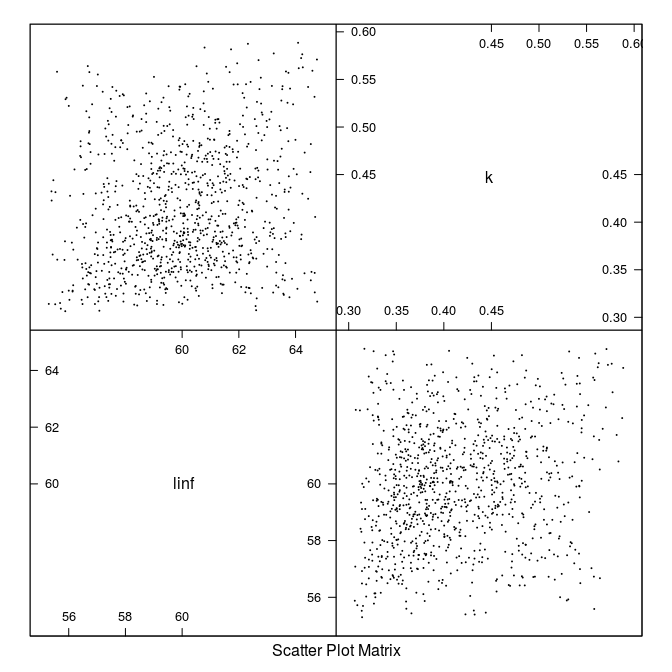
\includegraphics[width=.9\linewidth]{figure/plot_tri_gis_m-1} 

}

\caption[Parameter estimates for Gislason's second natural mortality model from using a triangle distribution]{Parameter estimates for Gislason's second natural mortality model from using a triangle distribution.}\label{fig:plot_tri_gis_m}
\end{figure}


\end{knitrout}

\begin{knitrout}
\definecolor{shadecolor}{rgb}{0.949, 0.949, 0.949}\color{fgcolor}\begin{figure}[H]

{\centering 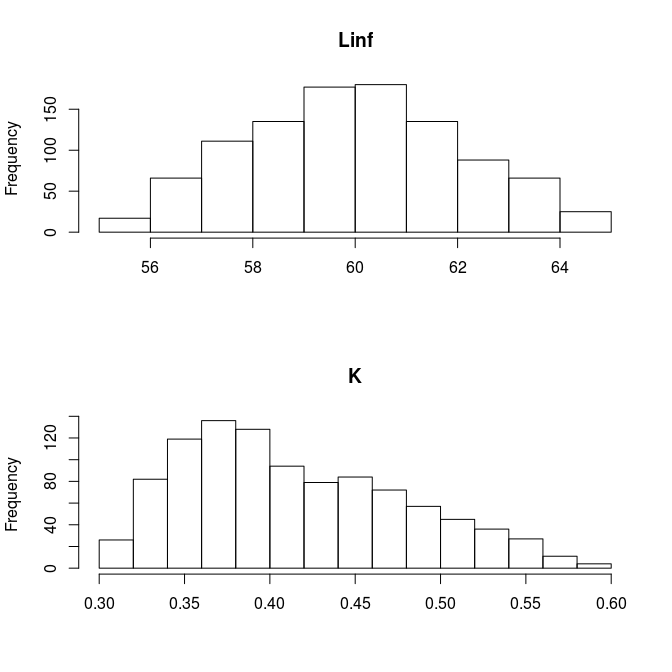
\includegraphics[width=.9\linewidth]{figure/plot_tri_gis_m_hist-1} 

}

\caption[Marginal distributions of the parameters for Gislason's second natural mortality model using a triangle distribution]{Marginal distributions of the parameters for Gislason's second natural mortality model using a triangle distribution.}\label{fig:plot_tri_gis_m_hist}
\end{figure}


\end{knitrout}

We now have a new model that can be used for the \code{shape} model. You can use the constructor or the set method to add the new model. Note that we have a quite complex method now for M. A length based \code{shape} model from Gislason's work, Jensen's third model based on temperature \code{level} and a time \code{trend} depending on NAO. All of the component models have uncertainty in their parameters.

\begin{knitrout}
\definecolor{shadecolor}{rgb}{0.949, 0.949, 0.949}\color{fgcolor}\begin{kframe}
\begin{alltt}
\hlstd{m5} \hlkwb{<-} \hlkwd{a4aM}\hlstd{(}\hlkwc{shape} \hlstd{= mgis2,} \hlkwc{level} \hlstd{= level4,} \hlkwc{trend} \hlstd{= trend4)}
\hlcom{# or}
\hlstd{m5} \hlkwb{<-} \hlstd{m4}
\hlkwd{shape}\hlstd{(m5)} \hlkwb{<-} \hlstd{mgis2}
\end{alltt}
\end{kframe}
\end{knitrout}

\section{Computing natural mortality time series - the "m" method}

Now that we have set up the natural mortality \class{a4aM} model and added parameter uncertainty to each component, we are ready to generate the \class{FLQuant} of natural mortality. For that we need the \code{m()} method.

The \code{m()} method is the workhorse method for computing natural mortality. The method returns an \class{FLQuant} that can be inserted in an \class{FLStock} for usage by the assessment method.

%The method uses the \code{range} slot to work out the dimensions of the \class{FLQuant} object. 
% Future developments will also allow for easy insertion into FLStockLen objects.

The size of the \class{FLQuant} object is determined by the \code{min}, \code{max}, \code{minyear} and \code{maxyear} elements of the \code{range} slot of the \class{a4aM} object. By default the values of these elements are set to 0. Giving an \class{FLQuant} with length 1 in the \code{quant} and \code{year} dimension. The \code{range} slot can be set by hand, or by using the \code{rngquant()} and \code{rngyear()} methods.

The name of the first dimension of the output \class{FLQuant} (e.g. 'age' or 'len') is determined by the parameters of the \code{shape} model. If it is not clear what the name should be then the name is set to 'quant'.

Here we demonstrate \code{m()} using the simple \class{a4aM} object we created above that has constant natural mortality.

Start with the simplest model:

\begin{knitrout}
\definecolor{shadecolor}{rgb}{0.949, 0.949, 0.949}\color{fgcolor}\begin{kframe}
\begin{alltt}
\hlstd{m1}
\end{alltt}
\begin{verbatim}
## a4aM object:
##   shape: ~1
##   level: ~a
##   trend: ~1
\end{verbatim}
\end{kframe}
\end{knitrout}

Check the range:

\begin{knitrout}
\definecolor{shadecolor}{rgb}{0.949, 0.949, 0.949}\color{fgcolor}\begin{kframe}
\begin{alltt}
\hlkwd{range}\hlstd{(m1)}
\end{alltt}
\begin{verbatim}
##       min       max plusgroup   minyear   maxyear   minmbar   maxmbar 
##         0         0         0         0         0         0         0
\end{verbatim}
\end{kframe}
\end{knitrout}

Simple - no ages or years:

\begin{knitrout}
\definecolor{shadecolor}{rgb}{0.949, 0.949, 0.949}\color{fgcolor}\begin{kframe}
\begin{alltt}
\hlkwd{m}\hlstd{(m1)}
\end{alltt}
\begin{verbatim}
## An object of class "FLQuant"
## , , unit = unique, season = all, area = unique
## 
##      year
## quant 0  
##     0 0.2
## 
## units:  NA
\end{verbatim}
\end{kframe}
\end{knitrout}

Set the quant and year ranges:

\begin{knitrout}
\definecolor{shadecolor}{rgb}{0.949, 0.949, 0.949}\color{fgcolor}\begin{kframe}
\begin{alltt}
\hlkwd{range}\hlstd{(m1,} \hlkwd{c}\hlstd{(}\hlstr{"min"}\hlstd{,} \hlstr{"max"}\hlstd{))} \hlkwb{<-} \hlkwd{c}\hlstd{(}\hlnum{0}\hlstd{,} \hlnum{7}\hlstd{)}  \hlcom{# set the quant range}
\hlkwd{range}\hlstd{(m1,} \hlkwd{c}\hlstd{(}\hlstr{"minyear"}\hlstd{,} \hlstr{"maxyear"}\hlstd{))} \hlkwb{<-} \hlkwd{c}\hlstd{(}\hlnum{2000}\hlstd{,} \hlnum{2010}\hlstd{)}  \hlcom{# set the year range}
\hlkwd{range}\hlstd{(m1)}
\end{alltt}
\begin{verbatim}
##       min       max plusgroup   minyear   maxyear   minmbar   maxmbar 
##         0         7         0      2000      2010         0         0
\end{verbatim}
\end{kframe}
\end{knitrout}

Create the object with the M estimates by age and year, note the name of the first dimension is 'quant'.

\begin{knitrout}
\definecolor{shadecolor}{rgb}{0.949, 0.949, 0.949}\color{fgcolor}\begin{kframe}
\begin{alltt}
\hlkwd{m}\hlstd{(m1)}
\end{alltt}
\begin{verbatim}
## , , unit = unique, season = all, area = unique
## 
##      year
## quant 2000 2001 2002 2003 2004
##     0 0.2  0.2  0.2  0.2  0.2 
##     1 0.2  0.2  0.2  0.2  0.2 
##     2 0.2  0.2  0.2  0.2  0.2 
##     3 0.2  0.2  0.2  0.2  0.2 
##     4 0.2  0.2  0.2  0.2  0.2 
##     5 0.2  0.2  0.2  0.2  0.2 
##     6 0.2  0.2  0.2  0.2  0.2 
##     7 0.2  0.2  0.2  0.2  0.2 
## 
##       [ ...  1 years]
## 
##      year
## quant 2006 2007 2008 2009 2010
##     0 0.2  0.2  0.2  0.2  0.2 
##     1 0.2  0.2  0.2  0.2  0.2 
##     2 0.2  0.2  0.2  0.2  0.2 
##     3 0.2  0.2  0.2  0.2  0.2 
##     4 0.2  0.2  0.2  0.2  0.2 
##     5 0.2  0.2  0.2  0.2  0.2 
##     6 0.2  0.2  0.2  0.2  0.2 
##     7 0.2  0.2  0.2  0.2  0.2
\end{verbatim}
\end{kframe}
\end{knitrout}

The next example has an age-based shape. As the \code{shape} model has 'age' as a variable which is not included in the \class{FLPar} slot it is used as the name of the first dimension of the resulting \class{FLQuant}. Note that in this case the \code{mbar} values in the range become relevant, once that \code{mbar} is used to compute the mean level. This mean level will match the value given by the \code{level} model. The \code{mbar} range can be changed with the \code{rngmbar()} method. We illustrate this by making an \class{FLQuant} with age varying natural mortality. 

Check the model and set the ranges:

\begin{knitrout}
\definecolor{shadecolor}{rgb}{0.949, 0.949, 0.949}\color{fgcolor}\begin{kframe}
\begin{alltt}
\hlstd{m2}
\end{alltt}
\begin{verbatim}
## a4aM object:
##   shape: ~exp(-age - 0.5)
##   level: ~1.5 * k
##   trend: ~1
\end{verbatim}
\begin{alltt}
\hlkwd{range}\hlstd{(m2,} \hlkwd{c}\hlstd{(}\hlstr{"min"}\hlstd{,} \hlstr{"max"}\hlstd{))} \hlkwb{<-} \hlkwd{c}\hlstd{(}\hlnum{0}\hlstd{,} \hlnum{7}\hlstd{)}  \hlcom{# set the quant range}
\hlkwd{range}\hlstd{(m2,} \hlkwd{c}\hlstd{(}\hlstr{"minyear"}\hlstd{,} \hlstr{"maxyear"}\hlstd{))} \hlkwb{<-} \hlkwd{c}\hlstd{(}\hlnum{2000}\hlstd{,} \hlnum{2003}\hlstd{)}  \hlcom{# set the year range}
\hlkwd{range}\hlstd{(m2)}
\end{alltt}
\begin{verbatim}
##       min       max plusgroup   minyear   maxyear   minmbar   maxmbar 
##         0         7         0      2000      2003         0         0
\end{verbatim}
\begin{alltt}
\hlkwd{m}\hlstd{(m2)}
\end{alltt}
\begin{verbatim}
## An object of class "FLQuant"
## , , unit = unique, season = all, area = unique
## 
##    year
## age 2000       2001       2002       2003      
##   0 0.60000000 0.60000000 0.60000000 0.60000000
##   1 0.22072766 0.22072766 0.22072766 0.22072766
##   2 0.08120117 0.08120117 0.08120117 0.08120117
##   3 0.02987224 0.02987224 0.02987224 0.02987224
##   4 0.01098938 0.01098938 0.01098938 0.01098938
##   5 0.00404277 0.00404277 0.00404277 0.00404277
##   6 0.00148725 0.00148725 0.00148725 0.00148725
##   7 0.00054713 0.00054713 0.00054713 0.00054713
## 
## units:  NA
\end{verbatim}
\end{kframe}
\end{knitrout}

Note that the level value is:

\begin{knitrout}
\definecolor{shadecolor}{rgb}{0.949, 0.949, 0.949}\color{fgcolor}\begin{kframe}
\begin{alltt}
\hlkwd{predict}\hlstd{(}\hlkwd{level}\hlstd{(m2))}
\end{alltt}
\begin{verbatim}
##    iter
##       1
##   1 0.6
\end{verbatim}
\end{kframe}
\end{knitrout}

Which is the same as:

\begin{knitrout}
\definecolor{shadecolor}{rgb}{0.949, 0.949, 0.949}\color{fgcolor}\begin{kframe}
\begin{alltt}
\hlkwd{m}\hlstd{(m2)[}\hlstr{"0"}\hlstd{]}
\end{alltt}
\begin{verbatim}
## An object of class "FLQuant"
## , , unit = unique, season = all, area = unique
## 
##    year
## age 2000 2001 2002 2003
##   0 0.6  0.6  0.6  0.6 
## 
## units:  NA
\end{verbatim}
\end{kframe}
\end{knitrout}

This is because the mbar range is currently set to "0" and "0" (see above) and the mean natural mortality value over this range is given by the level model. 

We can change the \code{mbar} range:

\begin{knitrout}
\definecolor{shadecolor}{rgb}{0.949, 0.949, 0.949}\color{fgcolor}\begin{kframe}
\begin{alltt}
\hlkwd{range}\hlstd{(m2,} \hlkwd{c}\hlstd{(}\hlstr{"minmbar"}\hlstd{,} \hlstr{"maxmbar"}\hlstd{))} \hlkwb{<-} \hlkwd{c}\hlstd{(}\hlnum{0}\hlstd{,} \hlnum{5}\hlstd{)}
\hlkwd{range}\hlstd{(m2)}
\end{alltt}
\begin{verbatim}
##       min       max plusgroup   minyear   maxyear   minmbar   maxmbar 
##         0         7         0      2000      2003         0         5
\end{verbatim}
\end{kframe}
\end{knitrout}

Which rescales the the natural mortality at age:

\begin{knitrout}
\definecolor{shadecolor}{rgb}{0.949, 0.949, 0.949}\color{fgcolor}\begin{kframe}
\begin{alltt}
\hlkwd{m}\hlstd{(m2)}
\end{alltt}
\begin{verbatim}
## An object of class "FLQuant"
## , , unit = unique, season = all, area = unique
## 
##    year
## age 2000      2001      2002      2003     
##   0 2.2812888 2.2812888 2.2812888 2.2812888
##   1 0.8392392 0.8392392 0.8392392 0.8392392
##   2 0.3087389 0.3087389 0.3087389 0.3087389
##   3 0.1135787 0.1135787 0.1135787 0.1135787
##   4 0.0417833 0.0417833 0.0417833 0.0417833
##   5 0.0153712 0.0153712 0.0153712 0.0153712
##   6 0.0056547 0.0056547 0.0056547 0.0056547
##   7 0.0020803 0.0020803 0.0020803 0.0020803
## 
## units:  NA
\end{verbatim}
\end{kframe}
\end{knitrout}

Check that the mortality over the mean range is the same as the level model:

\begin{knitrout}
\definecolor{shadecolor}{rgb}{0.949, 0.949, 0.949}\color{fgcolor}\begin{kframe}
\begin{alltt}
\hlkwd{quantMeans}\hlstd{(}\hlkwd{m}\hlstd{(m2)[}\hlkwd{as.character}\hlstd{(}\hlnum{0}\hlopt{:}\hlnum{5}\hlstd{)])}
\end{alltt}
\begin{verbatim}
## An object of class "FLQuant"
## , , unit = unique, season = all, area = unique
## 
##      year
## age   2000 2001 2002 2003
##   all 0.6  0.6  0.6  0.6 
## 
## units:  NA
\end{verbatim}
\end{kframe}
\end{knitrout}

The next example uses a time trend for the \code{trend} model. We use the \code{m3} model we made earlier. The \code{trend} model for this model has a covariate, 'nao'. This needs to be passed to the \code{m()} method. The year range of the 'nao' covariate should match that of the \code{range} slot.

Simple, pass in a single nao value (only one year):

\begin{knitrout}
\definecolor{shadecolor}{rgb}{0.949, 0.949, 0.949}\color{fgcolor}\begin{kframe}
\begin{alltt}
\hlkwd{m}\hlstd{(m3,} \hlkwc{nao} \hlstd{=} \hlnum{1}\hlstd{)}
\end{alltt}
\begin{verbatim}
## An object of class "FLQuant"
## , , unit = unique, season = all, area = unique
## 
##    year
## age 0  
##   0 0.9
## 
## units:  NA
\end{verbatim}
\end{kframe}
\end{knitrout}

Set ages:

\begin{knitrout}
\definecolor{shadecolor}{rgb}{0.949, 0.949, 0.949}\color{fgcolor}\begin{kframe}
\begin{alltt}
\hlkwd{range}\hlstd{(m3,} \hlkwd{c}\hlstd{(}\hlstr{"min"}\hlstd{,} \hlstr{"max"}\hlstd{))} \hlkwb{<-} \hlkwd{c}\hlstd{(}\hlnum{0}\hlstd{,} \hlnum{7}\hlstd{)}
\hlkwd{m}\hlstd{(m3,} \hlkwc{nao} \hlstd{=} \hlnum{0}\hlstd{)}
\end{alltt}
\begin{verbatim}
## An object of class "FLQuant"
## , , unit = unique, season = all, area = unique
## 
##    year
## age 0         
##   0 0.60000000
##   1 0.22072766
##   2 0.08120117
##   3 0.02987224
##   4 0.01098938
##   5 0.00404277
##   6 0.00148725
##   7 0.00054713
## 
## units:  NA
\end{verbatim}
\end{kframe}
\end{knitrout}

With ages and years - passing in the NAO data as numeric (1,0,1,0)

\begin{knitrout}
\definecolor{shadecolor}{rgb}{0.949, 0.949, 0.949}\color{fgcolor}\begin{kframe}
\begin{alltt}
\hlkwd{range}\hlstd{(m3,} \hlkwd{c}\hlstd{(}\hlstr{"minyear"}\hlstd{,} \hlstr{"maxyear"}\hlstd{))} \hlkwb{<-} \hlkwd{c}\hlstd{(}\hlnum{2000}\hlstd{,} \hlnum{2003}\hlstd{)}
\hlkwd{m}\hlstd{(m3,} \hlkwc{nao} \hlstd{=} \hlkwd{as.numeric}\hlstd{(nao[,} \hlkwd{as.character}\hlstd{(}\hlnum{2000}\hlopt{:}\hlnum{2003}\hlstd{)]))}
\end{alltt}
\begin{verbatim}
## An object of class "FLQuant"
## , , unit = unique, season = all, area = unique
## 
##    year
## age 2000       2001       2002       2003      
##   0 0.90000000 0.60000000 0.90000000 0.60000000
##   1 0.33109150 0.22072766 0.33109150 0.22072766
##   2 0.12180175 0.08120117 0.12180175 0.08120117
##   3 0.04480836 0.02987224 0.04480836 0.02987224
##   4 0.01648407 0.01098938 0.01648407 0.01098938
##   5 0.00606415 0.00404277 0.00606415 0.00404277
##   6 0.00223088 0.00148725 0.00223088 0.00148725
##   7 0.00082069 0.00054713 0.00082069 0.00054713
## 
## units:  NA
\end{verbatim}
\end{kframe}
\end{knitrout}

The final example show how \code{m()} can be used to make an \class{FLQuant} with uncertainty (see Figure~\ref{fig:uncertain_m}). We use the \code{m4} object from earlier with uncertainty on the \code{level} and \code{trend} parameters.

\begin{knitrout}
\definecolor{shadecolor}{rgb}{0.949, 0.949, 0.949}\color{fgcolor}\begin{kframe}
\begin{alltt}
\hlkwd{range}\hlstd{(m4,} \hlkwd{c}\hlstd{(}\hlstr{"min"}\hlstd{,} \hlstr{"max"}\hlstd{))} \hlkwb{<-} \hlkwd{c}\hlstd{(}\hlnum{0}\hlstd{,} \hlnum{7}\hlstd{)}
\hlkwd{range}\hlstd{(m4,} \hlkwd{c}\hlstd{(}\hlstr{"minyear"}\hlstd{,} \hlstr{"maxyear"}\hlstd{))} \hlkwb{<-} \hlkwd{c}\hlstd{(}\hlnum{2000}\hlstd{,} \hlnum{2003}\hlstd{)}
\hlstd{flq} \hlkwb{<-} \hlkwd{m}\hlstd{(m4,} \hlkwc{nao} \hlstd{=} \hlkwd{as.numeric}\hlstd{(nao[,} \hlkwd{as.character}\hlstd{(}\hlnum{2000}\hlopt{:}\hlnum{2003}\hlstd{)]))}
\hlstd{flq}
\end{alltt}
\begin{verbatim}
## An object of class "FLQuant"
## iters:  100 
## 
## , , unit = unique, season = all, area = unique
## 
##    year
## age 2000                2001                2002               
##   0 3.0296188(0.402945) 2.0102637(0.192625) 3.0296188(0.402945)
##   1 1.1145345(0.148235) 0.7395347(0.070863) 1.1145345(0.148235)
##   2 0.4100143(0.054533) 0.2720596(0.026069) 0.4100143(0.054533)
##   3 0.1508358(0.020061) 0.1000851(0.009590) 0.1508358(0.020061)
##   4 0.0554894(0.007380) 0.0368193(0.003528) 0.0554894(0.007380)
##   5 0.0204134(0.002715) 0.0135451(0.001298) 0.0204134(0.002715)
##   6 0.0075097(0.000999) 0.0049829(0.000477) 0.0075097(0.000999)
##   7 0.0027627(0.000367) 0.0018331(0.000176) 0.0027627(0.000367)
##    year
## age 2003               
##   0 2.0102637(0.192625)
##   1 0.7395347(0.070863)
##   2 0.2720596(0.026069)
##   3 0.1000851(0.009590)
##   4 0.0368193(0.003528)
##   5 0.0135451(0.001298)
##   6 0.0049829(0.000477)
##   7 0.0018331(0.000176)
## 
## units:  NA
\end{verbatim}
\begin{alltt}
\hlkwd{dim}\hlstd{(flq)}
\end{alltt}
\begin{verbatim}
## [1]   8   4   1   1   1 100
\end{verbatim}
\end{kframe}
\end{knitrout}

\begin{knitrout}
\definecolor{shadecolor}{rgb}{0.949, 0.949, 0.949}\color{fgcolor}\begin{figure}[H]

{\centering 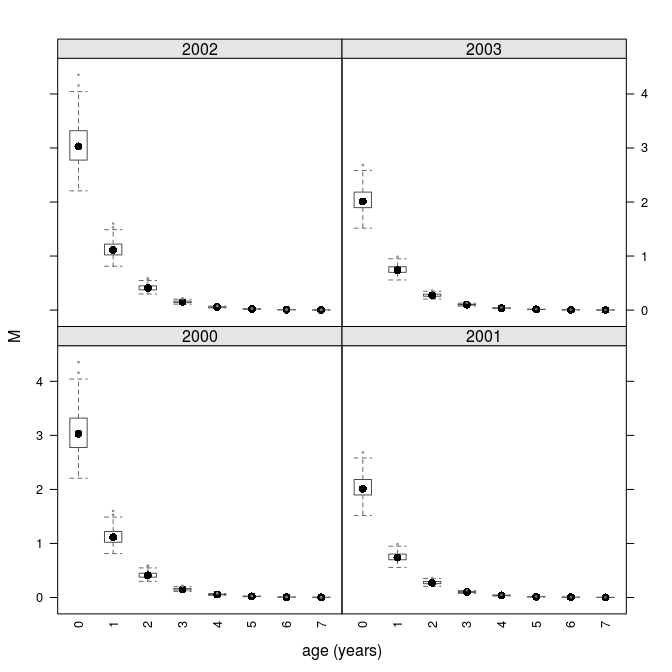
\includegraphics[width=.9\linewidth]{figure/uncertain_m-1} 

}

\caption[Natural mortality with age and year trend]{Natural mortality with age and year trend.}\label{fig:uncertain_m}
\end{figure}


\end{knitrout}

\end{document}

